%
% ---------------------------------------------------
%
% Proyecto de Final de Carrera:
% Author: Alejandro Hernández Padrón <alu0100703511@ull.edu.es>
% Capítulo: Objetivos 
% Fichero: Cap1_Goals.tex
%
% ----------------------------------------------------
%

\chapter{XXX Titulo capítulo} \label{chap:BeaconsEntornosUniversitarios}  


En este capítulo ...

 
\section{Aplicaciones móviles en entornos universitarios}


\begin{itemize}
\item XXX
\item XXX
\end{itemize}

\begin{figure}[h]
	\centering
	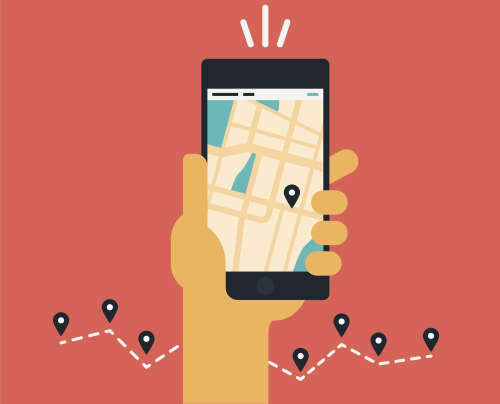
\includegraphics[width=0.6\linewidth]{locationMobileBeacon}
	\caption{Servicios de localización a través de la Universidad}
	\label{fig:beaconLocation}
\end{figure}

El funcionamiento sería el siguiente: el usuario transita por las inmediaciones del campus universitario. El usuario accede al sistema de navegación dentro de la aplicación, la cual le muestra entonces su ubicación como un punto de color sobre el mapa del campus. Este mapa tiene marcados puntos de interés que contienen información de diferente tipo dependiendo del punto marcado: nombre, historia, página web, teléfono de contacto, trámites asociados... son algunos de los datos que podría mostrar. El mapa se va actualizando dependiendo de la posición del usuario permitiendo volver a la vista más alejada en cualquier momento para una visualización más general.


\subsection{Descarga automática de material} \label{sec:descargaautomatica}



Otro posible uso de la tecnología beacon tiene que ver con las bibliotecas o lugares de almacenamiento de material. El estudiante se acercaría a la biblioteca buscando un libro específico. Partimos de que en la app estaría registrada la localización de los libros disponibles en los estantes. De esta manera la aplicación indicaría al alumno o alumna la posición del libro que busca. Para lugares amplios donde hay gran cantidad de material (véase la Figura \ref{fig:bibliotecaUSAL}), incluso podría guiar al usuario por las instalaciones hasta llegar a su objetivo, informarle del número de ejemplares disponibles o de la fecha prevista de entrada de algún título.

\begin{figure}[H]
	\centering
	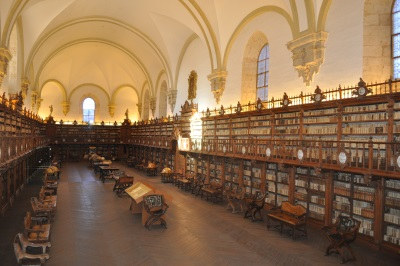
\includegraphics[width=0.6\linewidth]{BibliotecaSalamanca}
	\caption{La biblioteca de la Universidad de Salamanca contiene más de 1.000.000 de ejemplares lo que puede dificultar la localización de algunos títulos.}
	\label{fig:bibliotecaUSAL}
\end{figure}
